\documentclass[11pt]{article}

\usepackage[margin=1in]{geometry}
\usepackage{booktabs}
\usepackage{graphicx}
\usepackage{caption}
\usepackage{url}
\graphicspath{{figs lab 3/}}
\captionsetup{font=small, labelfont=bf}

\title{Workshop 3: Facial Expression Recognition on FER2013}
\author{Md Akmol Masud}
\date{November 10, 2026}

\begin{document}
\maketitle

% ---------------------------------------------------------------------------
\section{Setup}
All runs use FER2013 with FER+ labels (8 classes), a class-weighted loss, AdamW and the same augmentation. Because of the time limit, every arm trains for 8 epochs (16 for the longer-schedule arm) on a Colab T4. Macro-F1 is the main score; accuracy is for comparison with papers. Code and logs: \url{https://github.com/masud1901/elec-lab-3}

The classes are imbalanced (Figure~\ref{fig:counts}), so accuracy alone is misleading and macro-F1 is the right score.

\begin{figure}[h]
\centering
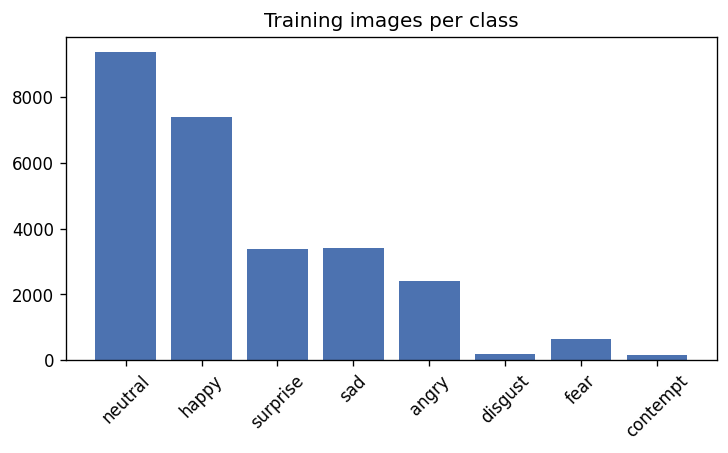
\includegraphics[width=0.48\linewidth]{class_counts.png}
\caption{Training images per class.}
\label{fig:counts}
\end{figure}

\begin{table}[h]
\centering
\small
\begin{tabular}{llccc}
\toprule
Ex. & Model & Test acc. & Test macro-F1 & Time (min) \\
\midrule
1 & ResNet-18, 128 px (baseline) & \textbf{0.841} & \textbf{0.694} & 3.1 \\
2 & ResNet-18, small stem, 48 px & 0.783 & 0.628 & 1.9 \\
3 & small stem + mixup/CutMix + EMA, 16 ep. & 0.778 & 0.648 & 3.2 \\
3 & EfficientNet-B0 + mixup + EMA, 128 px & 0.826 & 0.682 & 4.7 \\
4a & ResNet-18, no pretraining, 48 px & 0.742 & 0.557 & 1.9 \\
4b & AlexNet, 128 px & 0.785 & 0.613 & 3.9 \\
4d & ViT pretrained on expressions (validation only) & 0.697 & 0.501 & --- \\
\bottomrule
\end{tabular}
\caption{All experiments. Test numbers use the checkpoint with the best validation macro-F1.}
\label{tab:all}
\end{table}

% ---------------------------------------------------------------------------
\section{Exercise 1: Baseline}
The baseline is an ImageNet-pretrained ResNet-18 on faces enlarged to 128 px. It reaches test accuracy \textbf{0.841} and macro-F1 \textbf{0.694}, the best of all runs. Large classes score well (happy 0.93, surprise 0.88, neutral 0.86); rare classes score poorly (disgust 0.44, contempt 0.36, fear 0.56; Table~\ref{tab:perclass}). The main confusions are sad $\to$ neutral, disgust $\to$ angry, fear $\to$ surprise and contempt $\to$ neutral (Figure~\ref{fig:cm}).

\begin{table}[h]
\centering
\small
\begin{tabular}{lcccccccc}
\toprule
Model & neu. & hap. & sur. & sad & ang. & dis. & fear & con. \\
\midrule
Baseline (Ex.~1) & 0.858 & 0.934 & 0.876 & 0.707 & 0.808 & 0.444 & 0.564 & 0.357 \\
Small stem (Ex.~2) & 0.806 & 0.899 & 0.825 & 0.602 & 0.734 & 0.364 & 0.505 & 0.290 \\
Mixup/CutMix/EMA (Ex.~3) & 0.804 & 0.881 & 0.779 & 0.505 & 0.753 & 0.556 & 0.478 & 0.432 \\
EfficientNet-B0 (Ex.~3) & 0.848 & 0.914 & 0.844 & 0.672 & 0.800 & 0.400 & 0.538 & 0.439 \\
No pretraining (4a) & 0.776 & 0.861 & 0.811 & 0.531 & 0.679 & 0.286 & 0.383 & 0.125 \\
AlexNet (4b) & 0.809 & 0.899 & 0.830 & 0.597 & 0.738 & 0.318 & 0.462 & 0.245 \\
\bottomrule
\end{tabular}
\caption{Per-class test F1.}
\label{tab:perclass}
\end{table}

\begin{figure}[h]
\centering
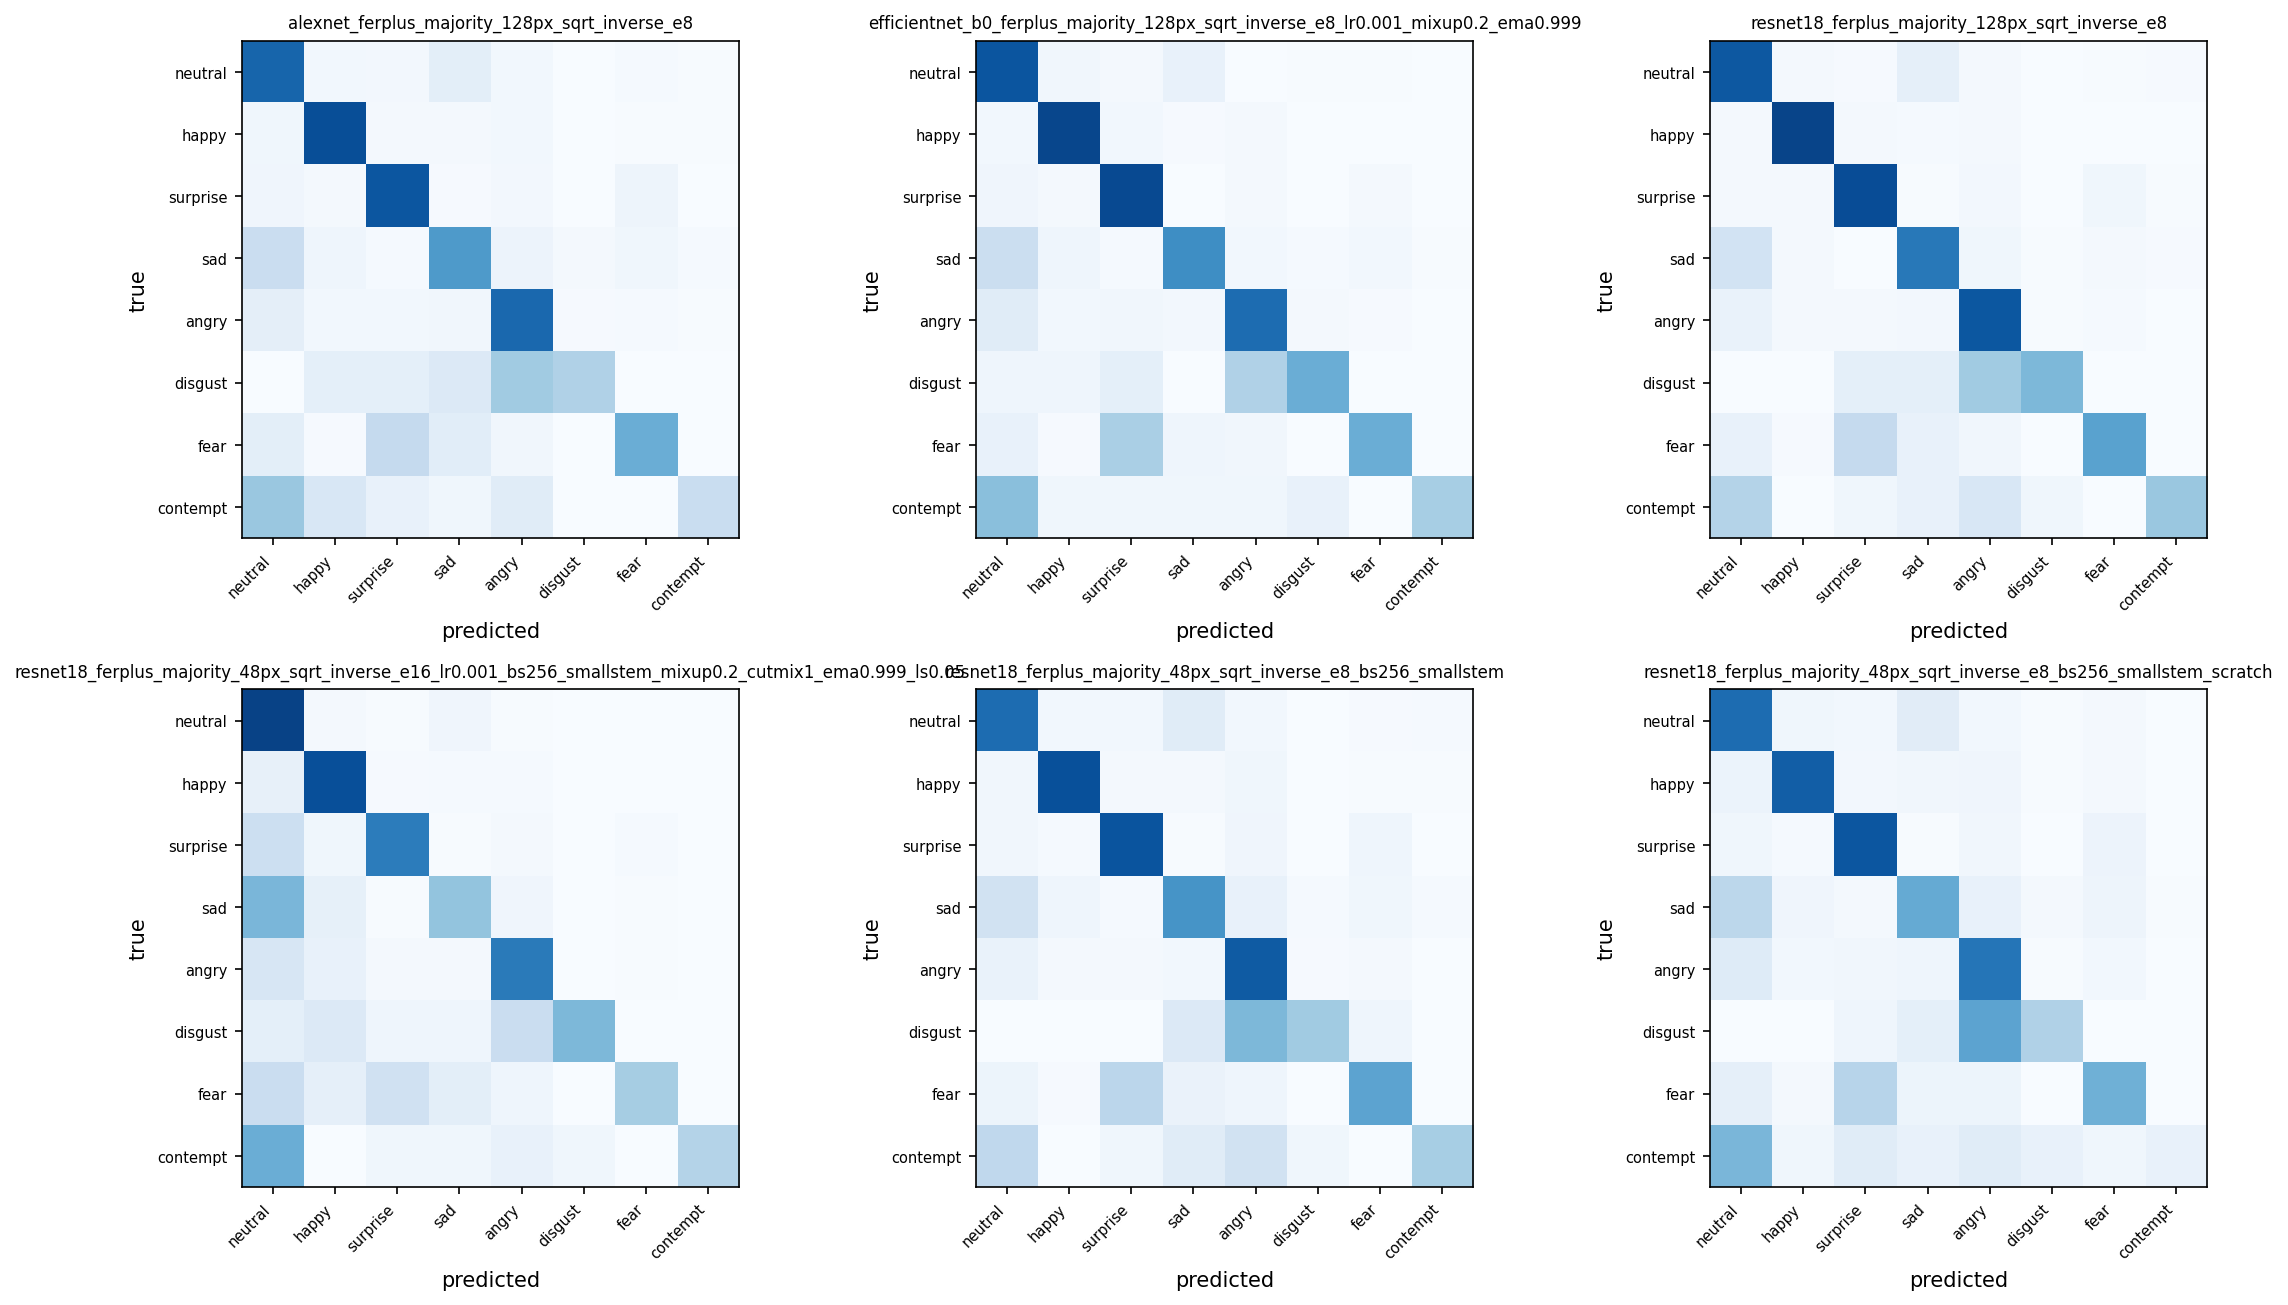
\includegraphics[width=\linewidth]{confusion_matrices_all.png}
\caption{Confusion matrices on the test set (rows: true class, columns: predicted).}
\label{fig:cm}
\end{figure}

% ---------------------------------------------------------------------------
\section{Exercise 2: Small images}
I keep the faces at 48 px and replace ResNet-18's 7$\times$7 stride-2 stem with a 3$\times$3 stride-1 convolution. The standard stem would shrink a 48 px face to 2$\times$2 in the last stage; the small stem keeps 24$\times$24 after the max-pool.

The small stem is worse than enlarging: accuracy 0.783 vs.\ 0.841 and macro-F1 0.628 vs.\ 0.694. It is faster (9~s vs.\ 15~s per epoch). The pretrained filters expect object scales of about 224 px, and the new first layer starts from scratch. The model was still improving at epoch 8, so a longer schedule would narrow the gap.

% ---------------------------------------------------------------------------
\section{Exercise 3: Improving the model}
Published single-network results on the original FER2013 labels are about 73\% accuracy (e.g.\ Khaireddin and Chen, 2021). % verify before submitting
They use the noisier original labels, so they do not compare directly with FER+.

My method combines three ideas: mixup (0.2) and CutMix (1.0), EMA of the weights (0.999), and a longer schedule (16 epochs) with learning rate $10^{-3}$. Mixup and CutMix blend images and labels so the network cannot memorise single faces. EMA evaluates a smoothed copy of the weights.

\begin{center}
\begin{tabular}{lcc}
\toprule
Model & Test acc. & Test macro-F1 \\
\midrule
Baseline, 128 px (Ex.~1) & 0.841 & 0.694 \\
Small stem, 48 px (Ex.~2) & 0.783 & 0.628 \\
Small stem + mixup/CutMix + EMA & 0.778 & 0.648 \\
EfficientNet-B0 + mixup + EMA, 128 px & 0.826 & 0.682 \\
\bottomrule
\end{tabular}
\end{center}

Against its own 48 px baseline, the method gains $+2.0$ points of macro-F1 and loses 0.5 points of accuracy. It does not beat the 128 px baseline. The gain comes from the rare classes (disgust 0.364 $\to$ 0.556, contempt 0.290 $\to$ 0.432) while sad and surprise get worse.

The method is under-trained, not over-regularised. With EMA 0.999 and 106 steps per epoch the averaged weights lag: validation accuracy is 0.26 after epoch 1, and the model is still improving at epoch 16 (Figure~\ref{fig:curves}). The exercise asks for 50--100 epochs; I trained 16. I did not run an ablation, so I do not know which component helped most.

% ---------------------------------------------------------------------------
\section{Exercise 4: Pretraining}

\paragraph{4a: No pretraining.} Accuracy 0.742, macro-F1 0.557. Against the same setup with ImageNet weights (Exercise 2), pretraining adds $+4.1$ points of accuracy and $+7.1$ of macro-F1. The gain is largest on rare classes (contempt 0.125 vs.\ 0.290).

\paragraph{4b: AlexNet.} Accuracy 0.785, macro-F1 0.613, against 0.841 / 0.694 for ResNet-18 at the same size.

\paragraph{4c: AlexNet vs.\ ResNet-18.}
\begin{figure}[h]
\centering
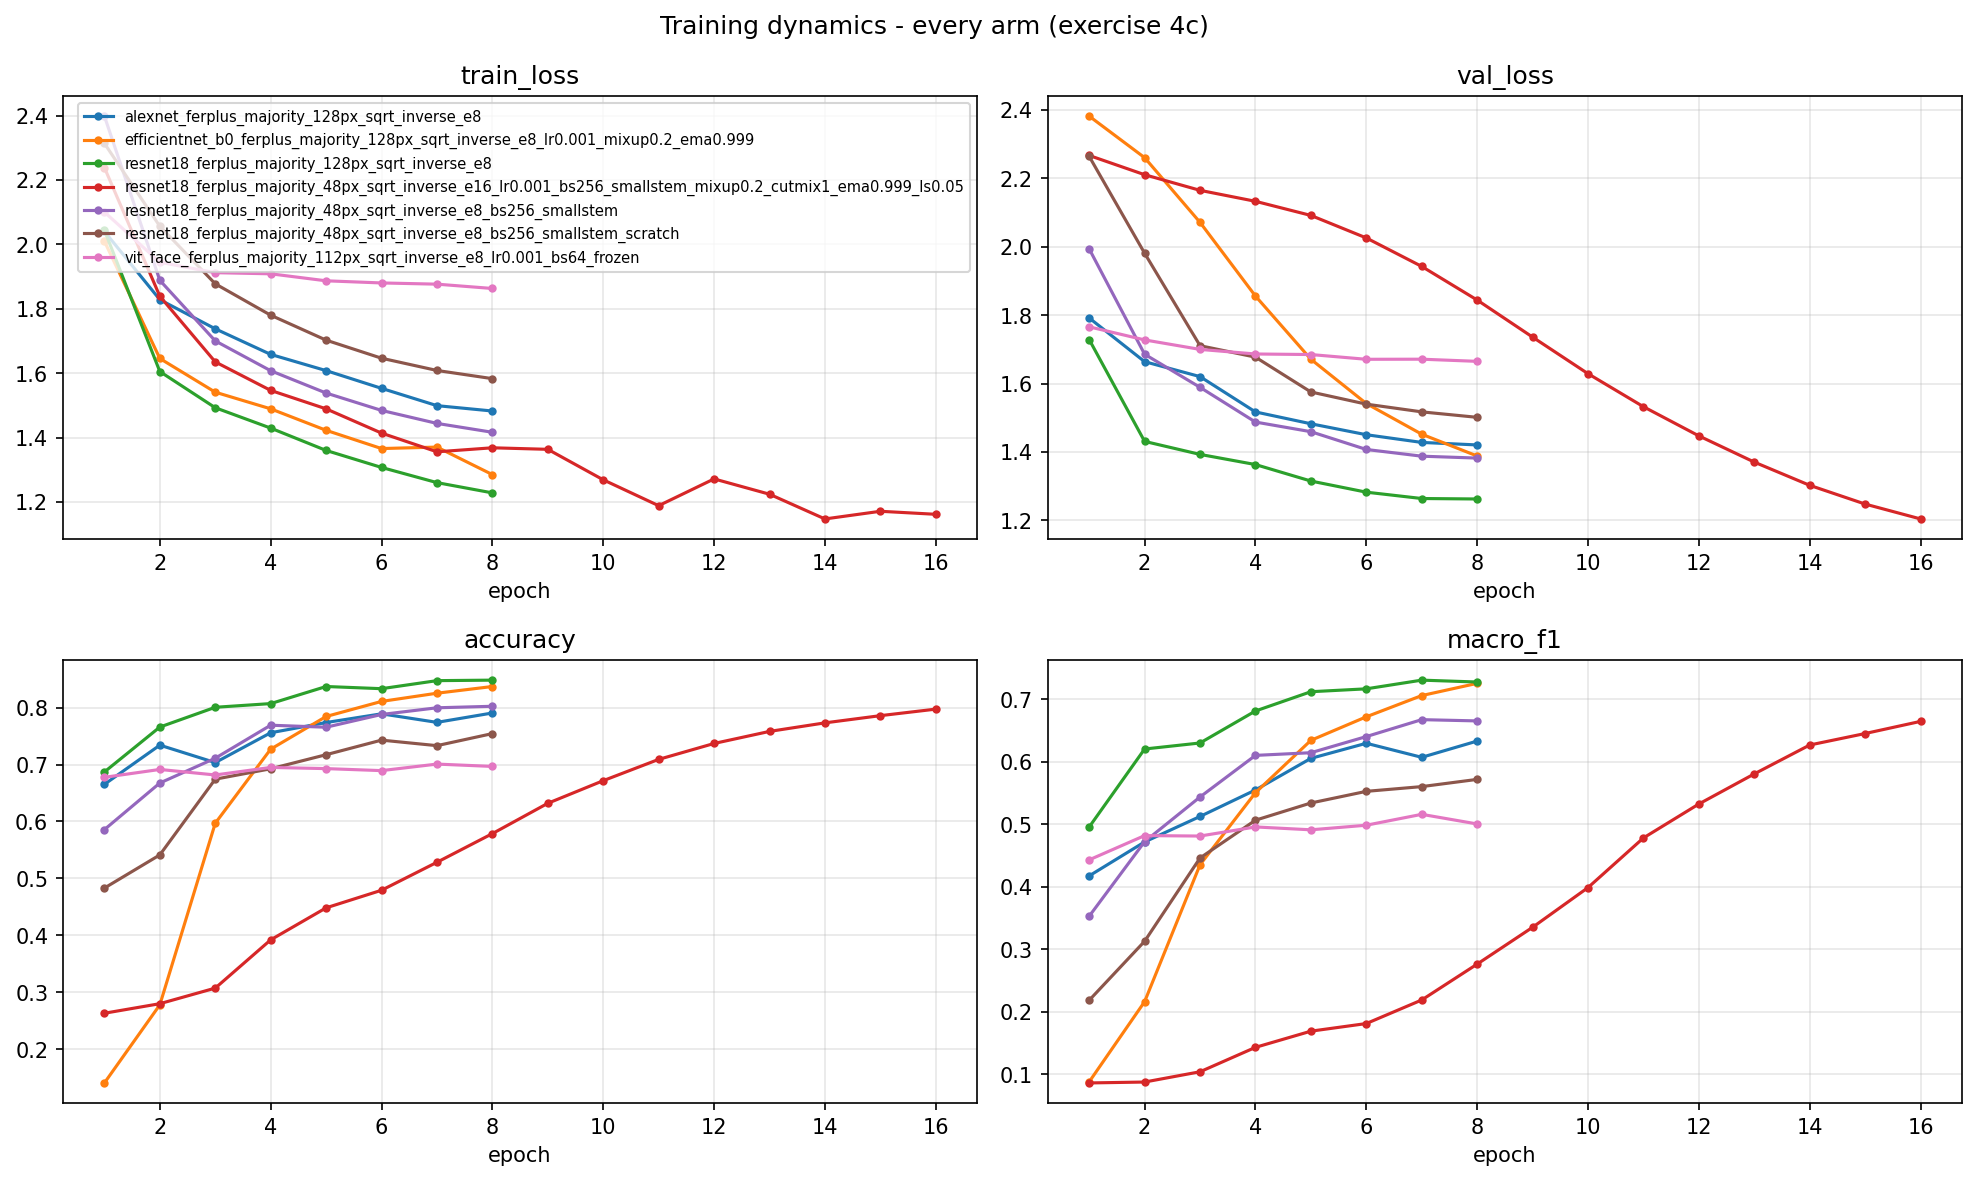
\includegraphics[width=\linewidth]{learning_curves_all.png}
\caption{Train loss, validation loss, validation accuracy and validation macro-F1 per epoch. ResNet-18: green. AlexNet: blue. No pretraining: brown. ViT: pink. Mixup/CutMix/EMA: red.}
\label{fig:curves}
\end{figure}
ResNet-18 is better at every epoch. After 8 epochs it has train loss 1.23 vs.\ 1.48, validation loss 1.26 vs.\ 1.42, validation accuracy 0.848 vs.\ 0.791 and validation macro-F1 0.728 vs.\ 0.633. AlexNet is also noisier. Neither network overfits in 8 epochs; the gap is optimisation speed. ResNet-18 has batch normalisation, residual connections and 11M parameters. AlexNet has no normalisation and 57M parameters, mostly in dense layers. I did not tune AlexNet's learning rate separately.

\paragraph{4d: Expression-pretrained network.} I use the ViT \texttt{trpakov/vit-face-expression}, pretrained on facial expressions, with a frozen encoder and a new head, at 112 px. Its test evaluation crashed on a bug in my code (fixed afterwards), so I report validation numbers: accuracy 0.697 and macro-F1 0.501. These are far below ResNet-18 (0.848 / 0.728) and not comparable to the test rows. The train loss stays at 1.86, so the model under-fits. The likely cause is the frozen encoder: only a small head adapts to the 8 FER+ classes. The checkpoint was also trained on FER2013, so it may have seen my test faces. Fine-tuning the encoder would be the next step.

% ---------------------------------------------------------------------------
\section{Exercise 5: Own photos}
I use the best model (ResNet-18, 128 px). The smiling photo is classified as \emph{happy} with 74\% confidence.

\begin{figure}[h]
\centering
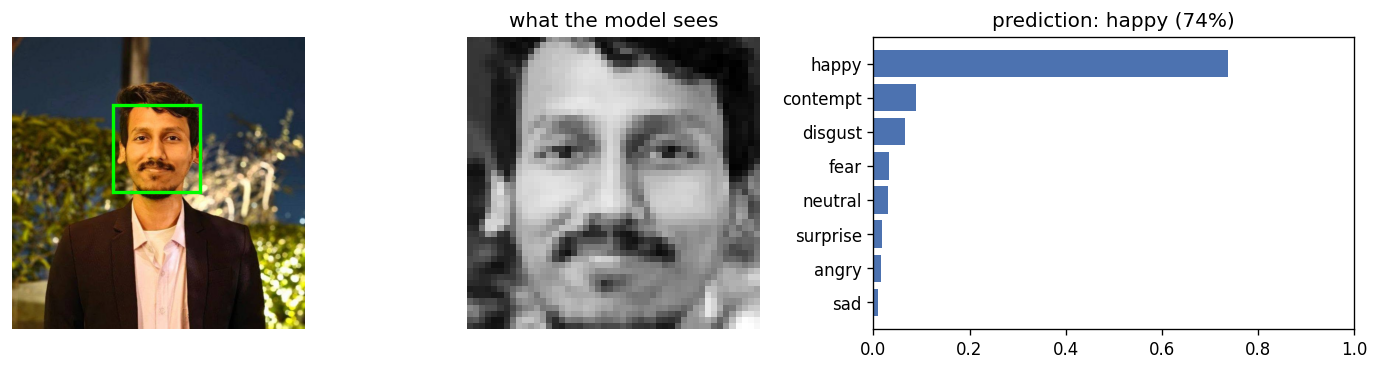
\includegraphics[width=\linewidth]{predictions_ayon.png}
\caption{Prediction for my photo: face found, \emph{happy} 74\%.}
\end{figure}

As a sanity check I use a cat picture. No face is found, yet the model answers \emph{sad} at only 25\%, with the probability spread across classes. The model always picks an expression; low confidence is the only warning.

\begin{figure}[h]
\centering
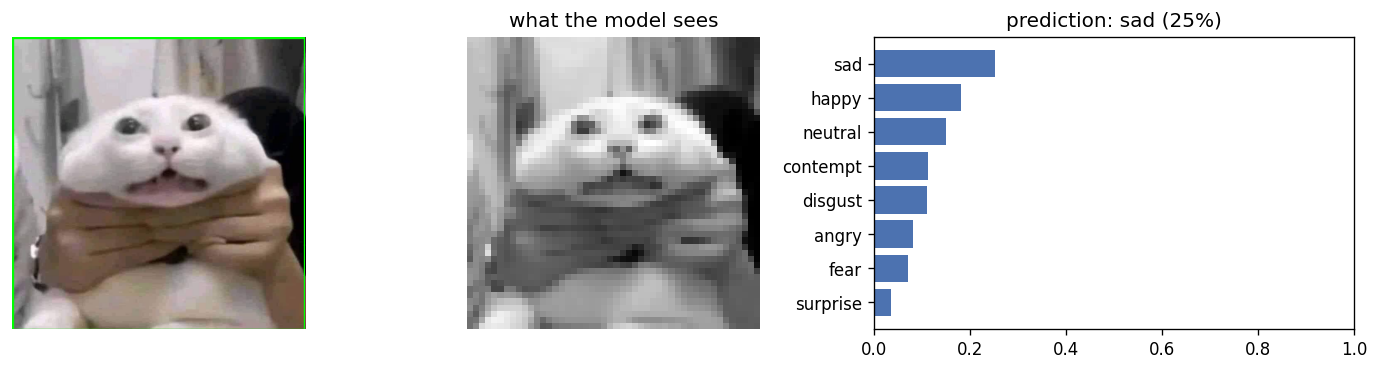
\includegraphics[width=\linewidth]{predictions_catto.png}
\caption{Prediction for a cat picture: no face found, \emph{sad} 25\%.}
\end{figure}

\section{Conclusions}
\begin{itemize}
\item Pretraining matters most: without it, macro-F1 drops by 7 points.
\item ResNet-18 beats AlexNet by 5.6 points of accuracy.
\item Enlarging 48 px faces beats the small stem, which is faster.
\item Mixup/CutMix/EMA helps rare classes but needs much longer training than I had.
\item A frozen expression-pretrained ViT does not beat ResNet-18.
\item Every result is one run with one seed; differences of one or two points are within noise.
\end{itemize}

\end{document}
